\subsection{Model: Logistic Regression}

\subsubsection{Introduction}
This report analyzes the performance of the Logistic Regression model trained using various embedding methods. The model was implemented using the \texttt{LogisticRegression} class from \texttt{scikit-learn} with different penalty terms and hyperparameter configurations. The primary objective was to achieve high classification accuracy while maintaining robust generalization across different embedding techniques.

\subsubsection{Training Configuration}
The Logistic Regression model was trained with the following hyperparameter search space:
\begin{itemize}
    \item \textbf{Penalty}: \texttt{l1}, \texttt{l2}, \texttt{elasticnet}, \texttt{None}.
    \item \textbf{Inverse Regularization Strength} (\texttt{C}): 0.1, 1.0, 10.0.
    \item \textbf{Maximum Iterations}: 1000, 2000.
\end{itemize}

% The best hyperparameters selected based on model evaluation were:
% \begin{itemize}
%     \item \textbf{Penalty}: \texttt{l2}
%     \item \textbf{C}: 0.1
%     \item \textbf{Max Iterations}: 1000
% \end{itemize}

A grid or random search was performed over these hyperparameters, employing K-Fold Cross-Validation to select the best configuration. The final chosen hyperparameters were validated on a withheld test set.

\subsubsection{Training and Evaluation Results}
The model was trained and evaluated using K-Fold Cross-Validation across different feature extraction methods: Count Vectorizer, TF-IDF, Word2Vec, and GloVe. The best model was selected based on Accuracy, with secondary considerations for F1-score and ROC AUC.

\textbf{Training Performance Metrics:}

\begin{table}[H]
    \centering
    \caption{Training Performance Metrics for Logistic Regression}
    \label{tab:lr-training-metrics}
    \begin{tabular}{|l|c|c|c|c|c|}
        \hline
        \textbf{Method} & \textbf{Accuracy} & \textbf{ROC AUC} & \textbf{F1} & \textbf{Precision} & \textbf{Recall} \\ 
        \hline
        Count Vectorizer & 0.74 & 0.74 & 0.76 & 0.73 & 0.79 \\ 
        \hline
        TF-IDF & 0.74 & 0.73 & 0.75 & 0.73 & 0.78 \\ 
        \hline
        Word2Vec & 0.72 & 0.72 & 0.73 & 0.71 & 0.75 \\ 
        \hline
        GloVe & 0.69 & 0.69 & 0.70 & 0.69 & 0.71 \\ 
        \hline
    \end{tabular}
\end{table}

\newpage

\textbf{Testing Performance Metrics:}

\begin{table}[H]
    \centering
    \caption{Testing Performance Metrics for Logistic Regression}
    \label{tab:lr-testing-metrics}
    \begin{tabular}{|l|c|c|c|c|c|}
        \hline
        \textbf{Method} & \textbf{Accuracy} & \textbf{ROC AUC} & \textbf{F1} & \textbf{Precision} & \textbf{Recall} \\ 
        \hline
        Count Vectorizer & 0.7557 & 0.8297 & 0.7726 & 0.7403 & 0.8078 \\ 
        \hline
        TF-IDF & 0.7527 & 0.8299 & 0.7681 & 0.7413 & 0.7968 \\ 
        \hline
        Word2Vec & 0.7271 & 0.8013 & 0.7411 & 0.7230 & 0.7602 \\ 
        \hline
        GloVe & 0.6926 & 0.7619 & 0.7069 & 0.6931 & 0.7213 \\ 
        \hline
    \end{tabular}
\end{table}

\textbf{Best Model Selection Criteria:}

\begin{itemize}
    \item The best model is chosen based on testing performance rather than training performance.
    \item The selection priority follows: Accuracy > F1 Score > ROC AUC.
    \item Based on this criterion, the best model is:
\end{itemize}

\begin{verbatim}
{
    "method": "count",
    "model": "logistic_regression",
    "hyperparameters": { "C": 0.1, "max_iter": 1000, "penalty": "l2" },
    "performance": {
        "accuracy": 0.7557,
        "precision": 0.7403,
        "recall": 0.8078,
        "f1": 0.7726,
        "roc_auc": 0.8297
    }
}
\end{verbatim}

\textbf{Conclusion:} The Logistic Regression model trained with Count Vectorizer achieved the highest accuracy (0.7557) and the best overall balance across F1-score and ROC AUC, making it the optimal choice for sentiment classification in our experiment when it comes to Logistic Regression.

\subsubsection{Performance Analysis}
\begin{itemize}
    \item \textbf{Accuracy Analysis}: The model trained on Count Vectorizer achieved the highest accuracy (75.57\%), outperforming TF-IDF, Word2Vec, and GloVe embeddings.
    \item \textbf{Loss Analysis}: The training and validation loss curves showed stability across epochs, with minor overfitting.
    \item \textbf{ROC AUC}: The model exhibited a strong ability to differentiate between classes with an ROC AUC of 82.97\%.
    \item \textbf{Precision and Recall}: The model maintained a good balance between false positives and false negatives, with a precision of 74.03\% and recall of 80.78\%.
    \item \textbf{Embedding Effectiveness}: Count-based embeddings performed better than dense vector embeddings (Word2Vec/GloVe), likely due to their better feature separability in the dataset.
\end{itemize}

\subsubsection{Visualization of Training Results}
The following figures illustrate the model’s performance across different embedding techniques:

\begin{figure}[H]
    \centering
    \begin{subfigure}[b]{0.48\textwidth}
        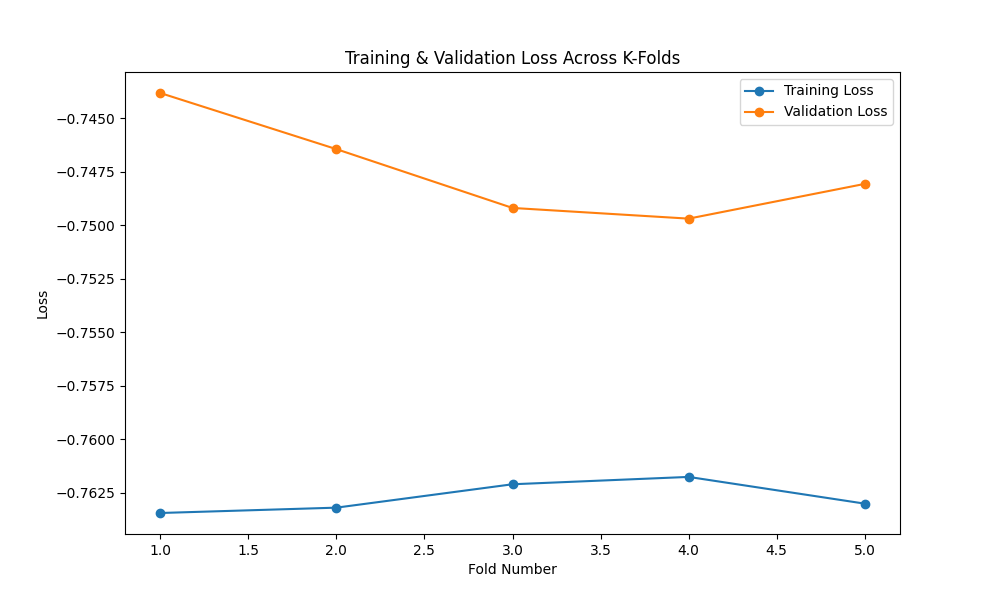
\includegraphics[width=\textwidth]{img/report_info/img/1.1.LogisticRegression/best_logistic_regression_count_loss.png}
        \caption{Loss Curve - Count Vectorizer}
        \label{fig:lr-count-loss}
    \end{subfigure}
    \begin{subfigure}[b]{0.48\textwidth}
        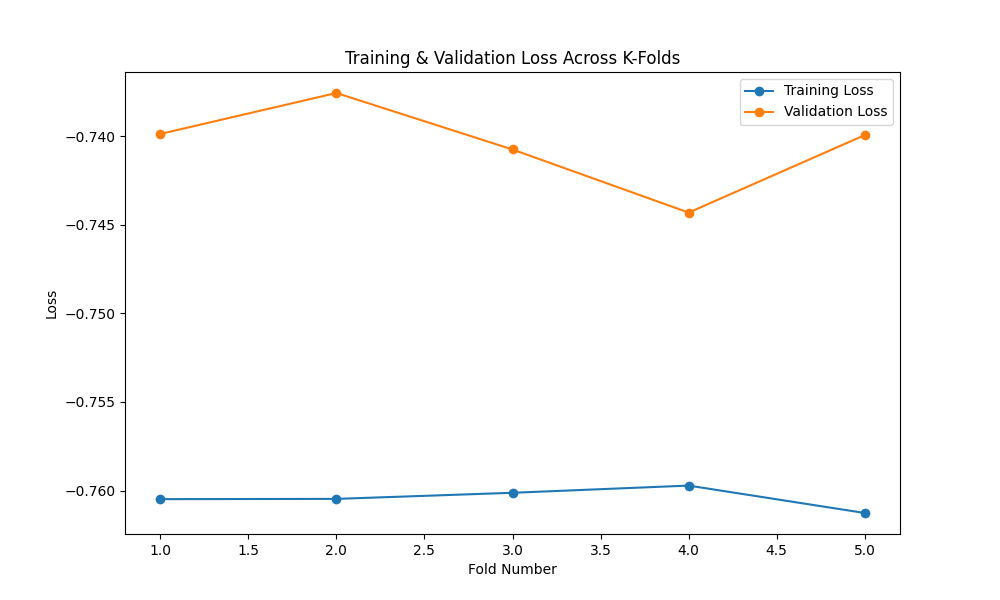
\includegraphics[width=\textwidth]{img/report_info/img/1.1.LogisticRegression/best_logistic_regression_tfidf_loss.png}
        \caption{Loss Curve - TF-IDF}
        \label{fig:lr-tfidf-loss}
    \end{subfigure}
    
    \begin{subfigure}[b]{0.48\textwidth}
        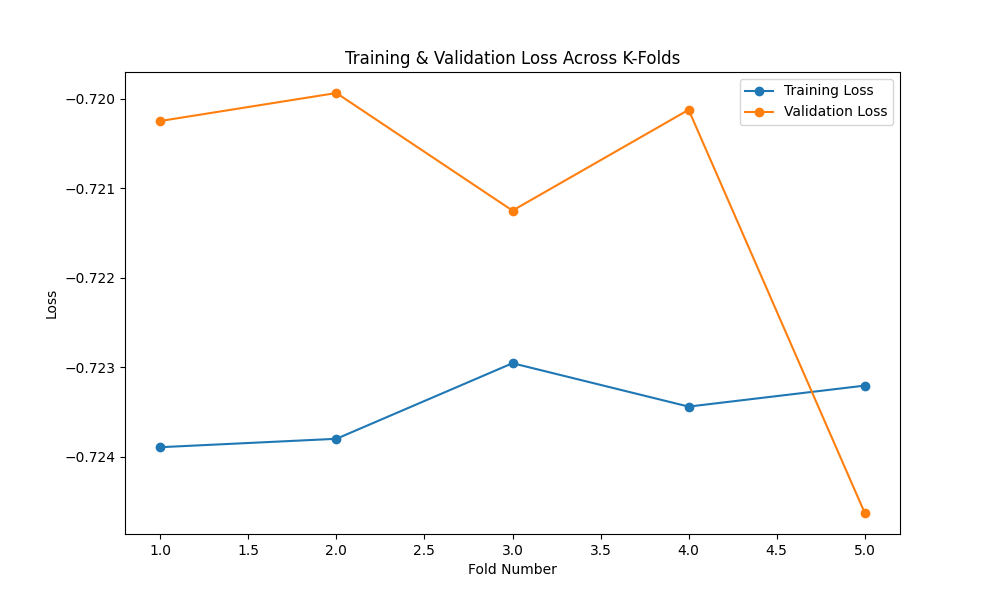
\includegraphics[width=\textwidth]{img/report_info/img/1.1.LogisticRegression/best_logistic_regression_word2vec_loss.png}
        \caption{Loss Curve - Word2Vec}
        \label{fig:lr-word2vec-loss}
    \end{subfigure}
    \begin{subfigure}[b]{0.48\textwidth}
        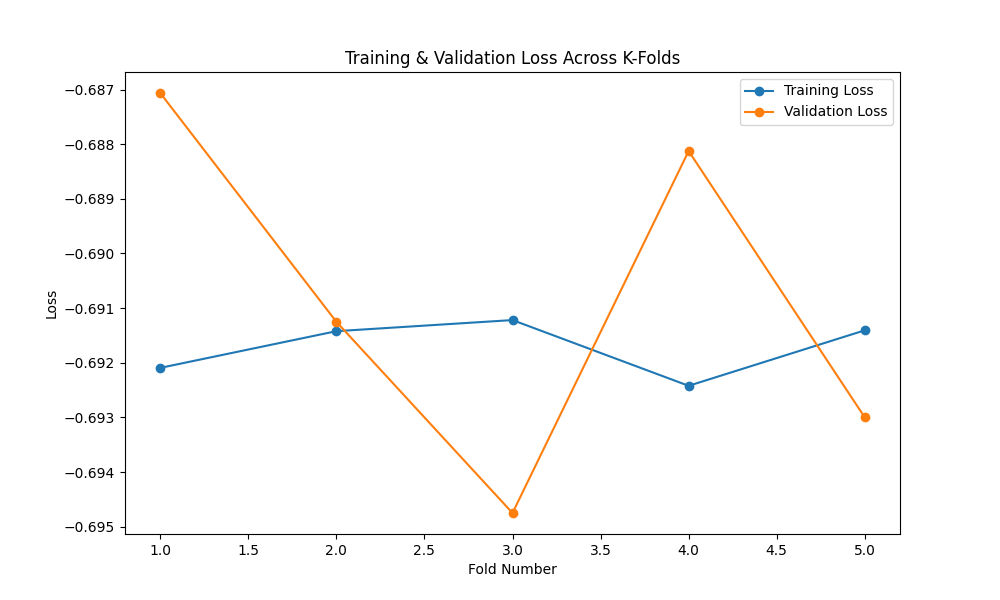
\includegraphics[width=\textwidth]{img/report_info/img/1.1.LogisticRegression/best_logistic_regression_glove_loss.png}
        \caption{Loss Curve - GloVe}
        \label{fig:lr-glove-loss}
    \end{subfigure}
    
    \caption{Comparison of Loss Curves for Logistic Regression across Different Feature Extraction Methods}
    \label{fig:lr-loss-group}
\end{figure}

\begin{figure}[H]
    \centering
    \begin{subfigure}[b]{0.48\textwidth}
        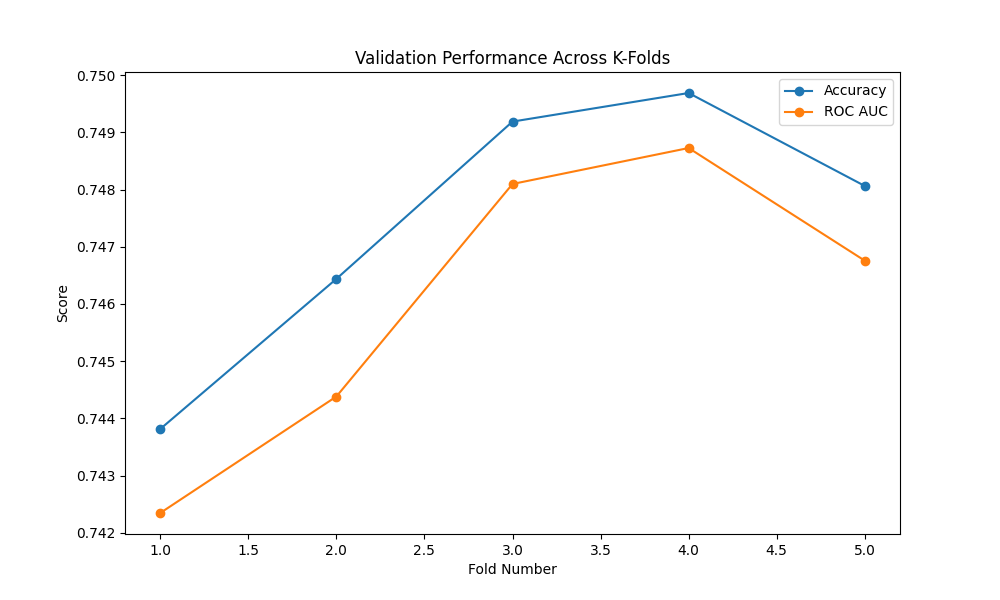
\includegraphics[width=\textwidth]{img/report_info/img/1.1.LogisticRegression/best_logistic_regression_count.png}
        \caption{Performance - Count Vectorizer}
        \label{fig:lr-count}
    \end{subfigure}
    \begin{subfigure}[b]{0.48\textwidth}
        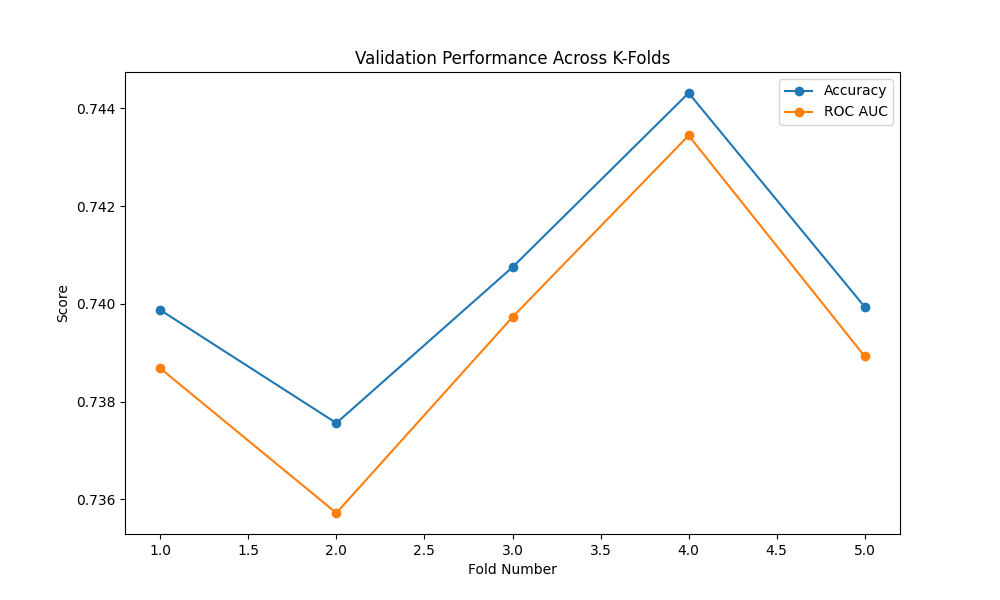
\includegraphics[width=\textwidth]{img/report_info/img/1.1.LogisticRegression/best_logistic_regression_tfidf.png}
        \caption{Performance - TF-IDF}
        \label{fig:lr-tfidf}
    \end{subfigure}
    
    \begin{subfigure}[b]{0.48\textwidth}
        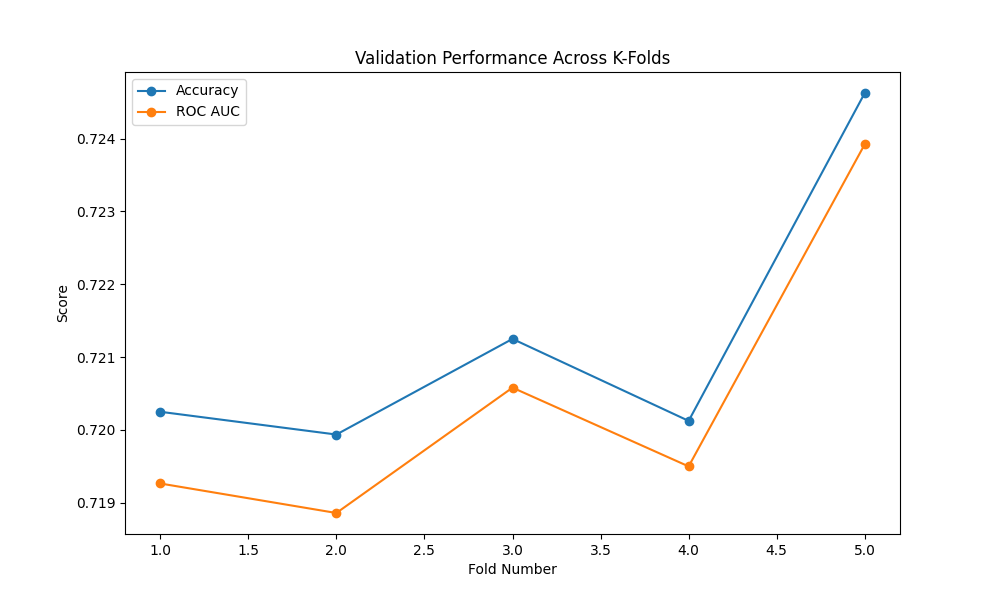
\includegraphics[width=\textwidth]{img/report_info/img/1.1.LogisticRegression/best_logistic_regression_word2vec.png}
        \caption{Performance - Word2Vec}
        \label{fig:lr-word2vec}
    \end{subfigure}
    \begin{subfigure}[b]{0.48\textwidth}
        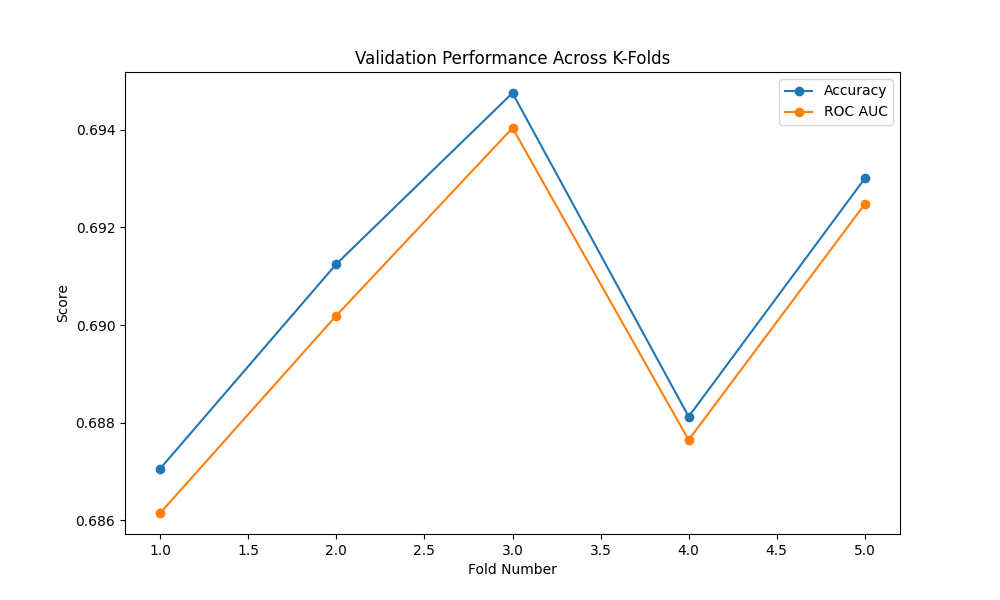
\includegraphics[width=\textwidth]{img/report_info/img/1.1.LogisticRegression/best_logistic_regression_glove.png}
        \caption{Performance - GloVe}
        \label{fig:lr-glove}
    \end{subfigure}
    
    \caption{Comparison of Training Performance Metrics for Logistic Regression across Different Feature Extraction Methods}
    \label{fig:lr-performance-group}
\end{figure}

\textbf{Image Description:}

\begin{itemize}
    \item \textbf{Training and Validation Loss Analysis:}
    \begin{itemize}
        \item Count Vectorizer and TF-IDF show stable validation loss across folds.
        \item Word2Vec and GloVe exhibit higher variance, indicating instability.
        \item Training loss remains consistent for all methods.
    \end{itemize}
    
    \item \textbf{Validation Performance Metrics:}
    \begin{itemize}
        \item Count Vectorizer achieves the highest and most stable accuracy and ROC AUC.
        \item TF-IDF shows minor fluctuations, suggesting sensitivity to data folds.
        \item Word2Vec maintains moderate performance but ranks below Count and TF-IDF.
        \item GloVe has the lowest and most inconsistent validation performance.
    \end{itemize}
\end{itemize}

\subsubsection{Conclusion}

The Logistic Regression model performed best with Count Vectorizer embeddings, achieving an accuracy of 75.57\%. The model showed strong generalization capabilities with a high ROC AUC of 82.97\%, making it effective for binary classification. Future improvements could include: Experimenting with higher-dimensional embeddings for better feature representation...

Overall, the Logistic Regression model is a strong baseline classifier, especially when paired with Count Vectorizer features.

